\chapter{Opis działania aplikacji}

Rozdział opisuje logikę funkcjonowania aplikacji poprzez opisanie jej poszczególnych funkcjonalności oraz przedstawienie kodu.

\section{Środowisko i narzędzia}
\begin{itemize}
    \item Android Studio,
    \item Język Java,
    \item ESP32 - Arduino IDE,
    \item XAMPP (Apache, MySQL),
    \item Docker
\end{itemize}

\section{Struktura projektu}
Struktura projektu składa się z plików projektu aplikacji Android Studio, projektu aplikacji serwera SpringBoot w IntelliJ, oraz bazy danych implementowanej za pomocą Docker Desktop.

\section{Interfejs użytkownika}

Sekcja "Aktualna Temperatura": Umieszczona na samej górze wewnątrz karty. Wyświetla największą czcionką ostatni odczyt z bazy danych, co pozwala na natychmiastowe sprawdzenie stanu termometru.

Sekcja "Historia zapisów": Poniżej karty znajduje się dynamiczna lista. Każdy wiersz zawiera temperaturę oraz dokładną datę i godzinę wykonania pomiaru. \\

\pagebreak

Jak pokazano na rysunku \ref{fig:schemat_png}, poniżej interfejs został zaprojektowany z myślą o czytelności i nowoczesnym wyglądzie.
\begin{figure}[H]
    \centering
    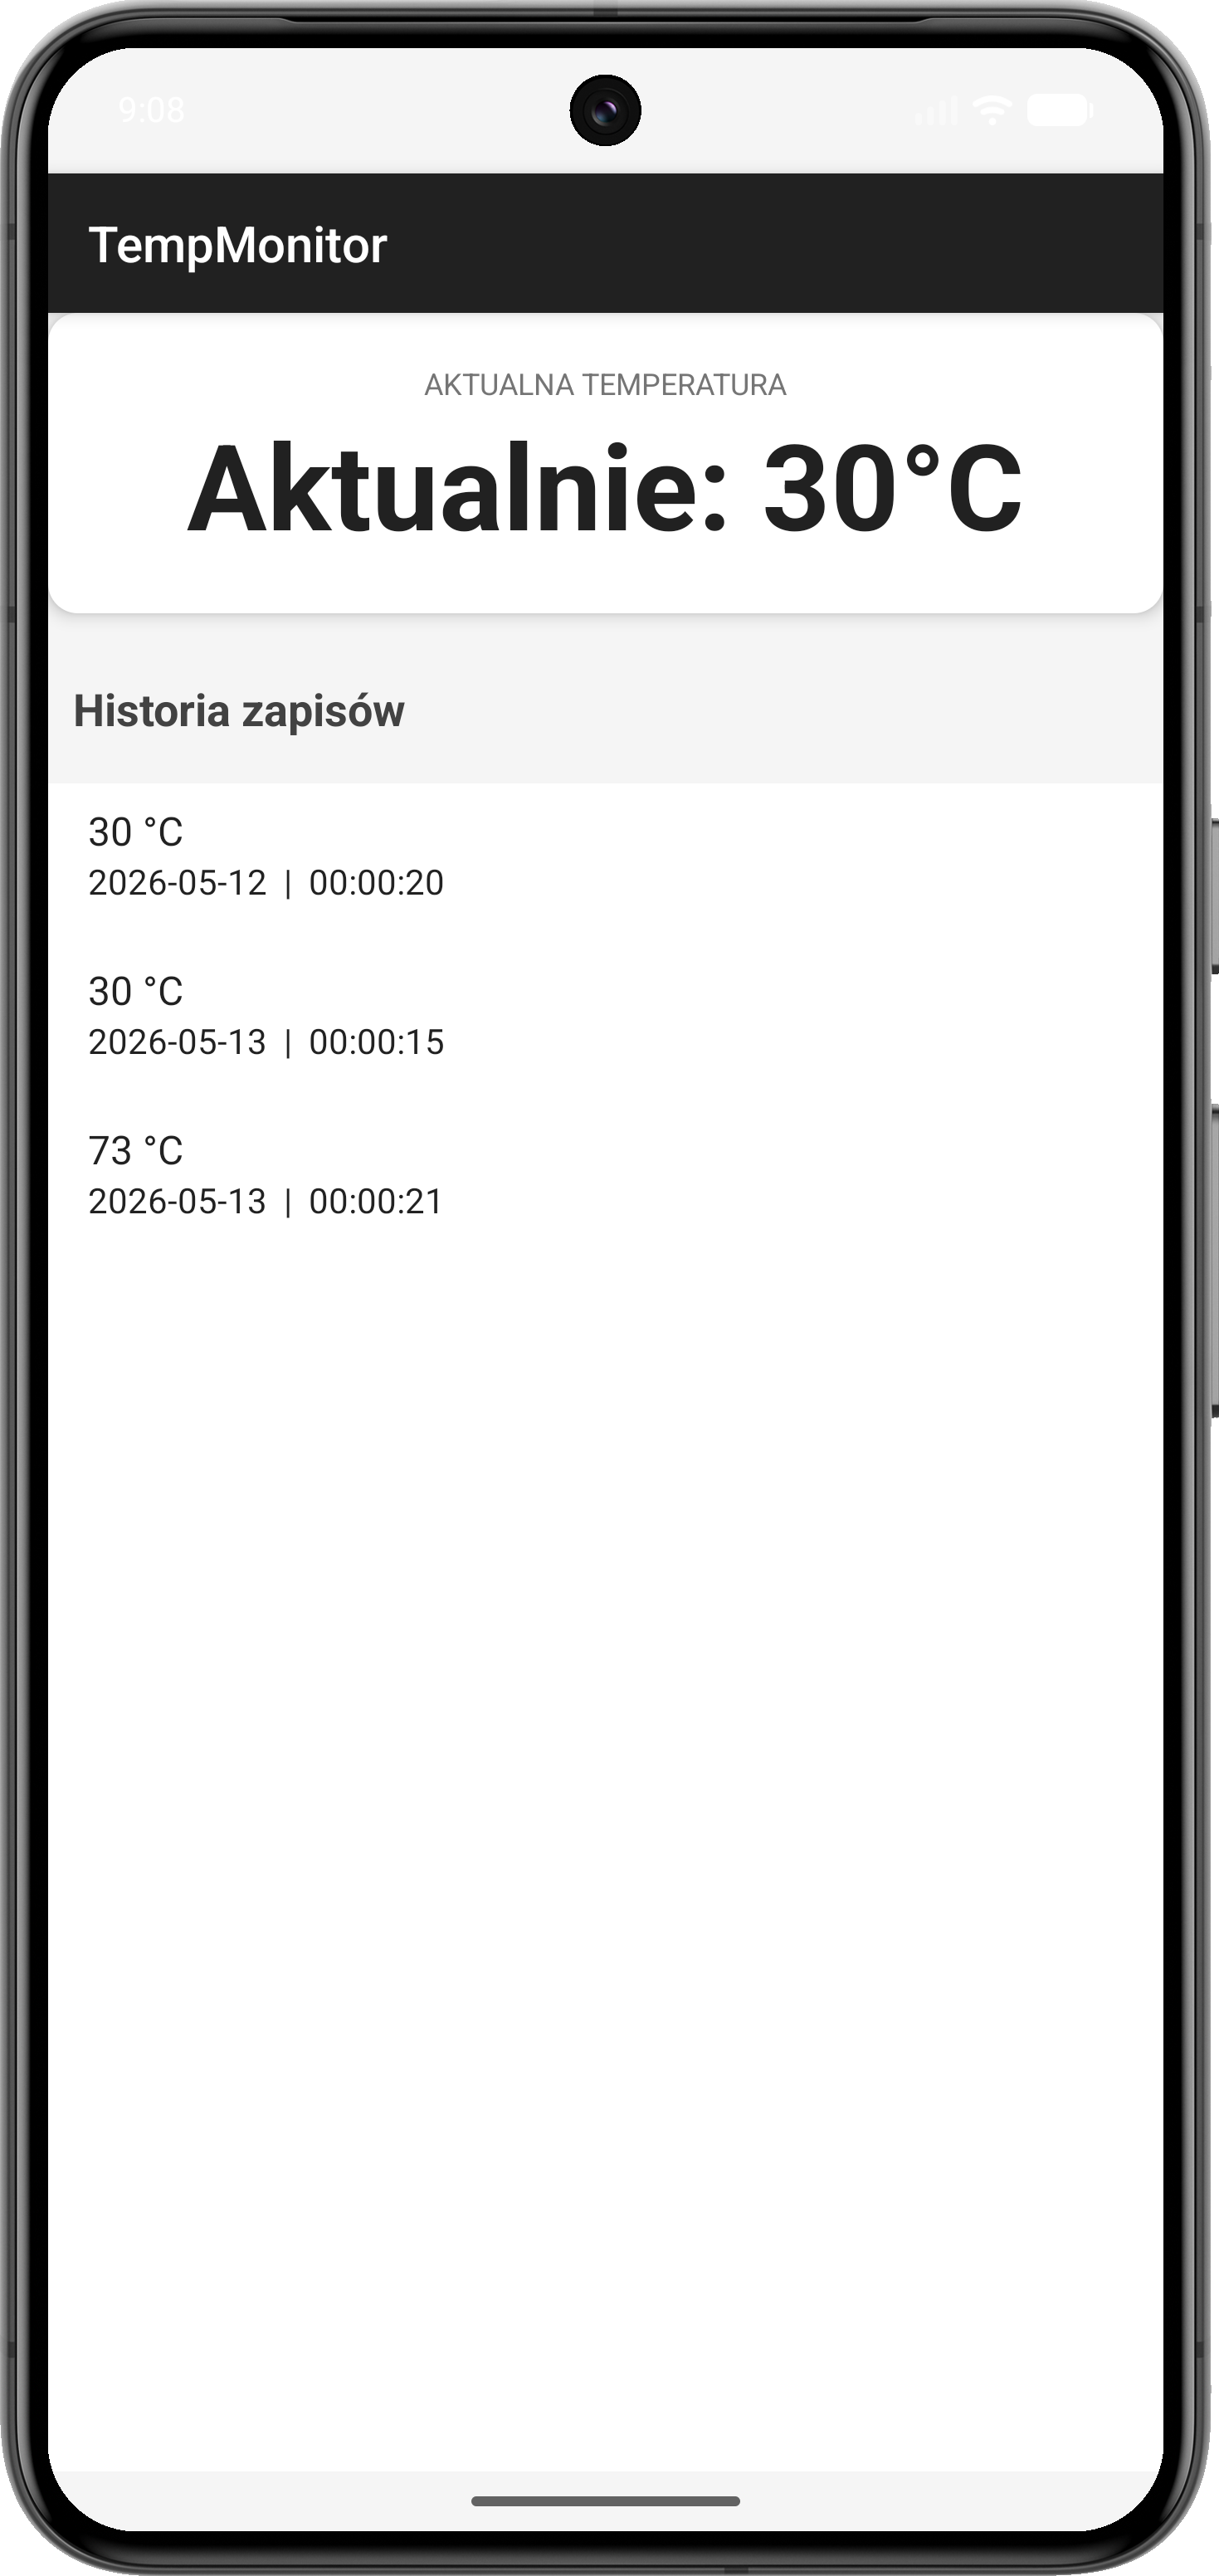
\includegraphics[width=0.6\textwidth]{rysunki/1.png} 
    \caption{Interface aplikacji}
    \label{fig:schemat_png} % Klucz dla grafiki PNG
    \sourcefig{opracowanie własne przy użyciu emulatora Android Studio}
\end{figure}

\section{Pobieranie danych z REST API}
Aplikacja korzysta z biblioteki Retrofit do asynchronicznego pobierania danych. Oznacza to, że pobieranie odbywa się w tle i nie zawiesza ekranu użytkownika.
\begin{lstlisting}[language=Java, caption={Pobieranie danych z API (Fragment ApiService.java)}]
@GET("api/pomiary")
Call<List<Dane>> getWszystkiePomiary();
\end{lstlisting}

\section{Automatyczne odświeżanie co 10 sekund}
Zastosowano mechanizm Handler i Runnable, który tworzy pętlę czasową. Funkcja ta jest inteligentna: uruchamia się, gdy aplikacja jest widoczna, i zatrzymuje, gdy użytkownik ją zminimalizuje.
\begin{lstlisting}[language=Java, caption={Odświeżanie (Fragment MainActivity.java)}]
    refreshRunnable = new Runnable() {
    @Override
    public void run() {
        pobierzDaneZSerwera(); // Wywołanie API
        handler.postDelayed(this, 10000); // Ponowne uruchomienie za 10s
    }
};       
\end{lstlisting}

\section{Logika wyświetlania aktualnej temperatury}
Aplikacja nie potrzebuje osobnego zapytania o jedną temperaturę. Pobiera całą listę, a następnie wybiera z niej ostatni element, aby wyświetlić go jako stan aktualny.
\begin{lstlisting}[language=Java, caption={Wyswietlanie "Aktualnej temperatury" (Fragment MainActivity.java)}]
    if (!daneList.isEmpty()) {
    Dane ostatni = daneList.get(daneList.size() - 1); // Pobranie najnowszego wpisu
    tvCurrentTemp.setText(ostatni.getTemperatura() + "'C");
    Collections.reverse(daneList); // Odwrocenie listy dla historii (najnowsze na gorze)
}
\end{lstlisting}

\section{Wyświetlanie dziennika}
Adapter bierze surowe dane i wstrzykuje je w odpowiednie pola tekstowe w layoucie.
\begin{lstlisting}[language=Java, caption={Wyswietlanie diennika (Fragment DaneAdapter.java)}]
    @Override
    public void onBindViewHolder(@NonNull ViewHolder holder, int position) {
    Dane d = lista.get(position);
    holder.text1.setText(d.getTemperatura() + "'C");
    holder.text2.setText(d.getData() + "  |  " + d.getGodzina());
}
\end{lstlisting}